% !TEX root = ../../semexp-thesis.tex

\section{Semantic Completions}
\label{sec:implementation/completions}

Our implementation of semantic completions reuses the framework of the suggestion space for tracking the experiments of programmers.

% todo: decide after planning application which figures make sense here
\begin{figure}
	\centering
	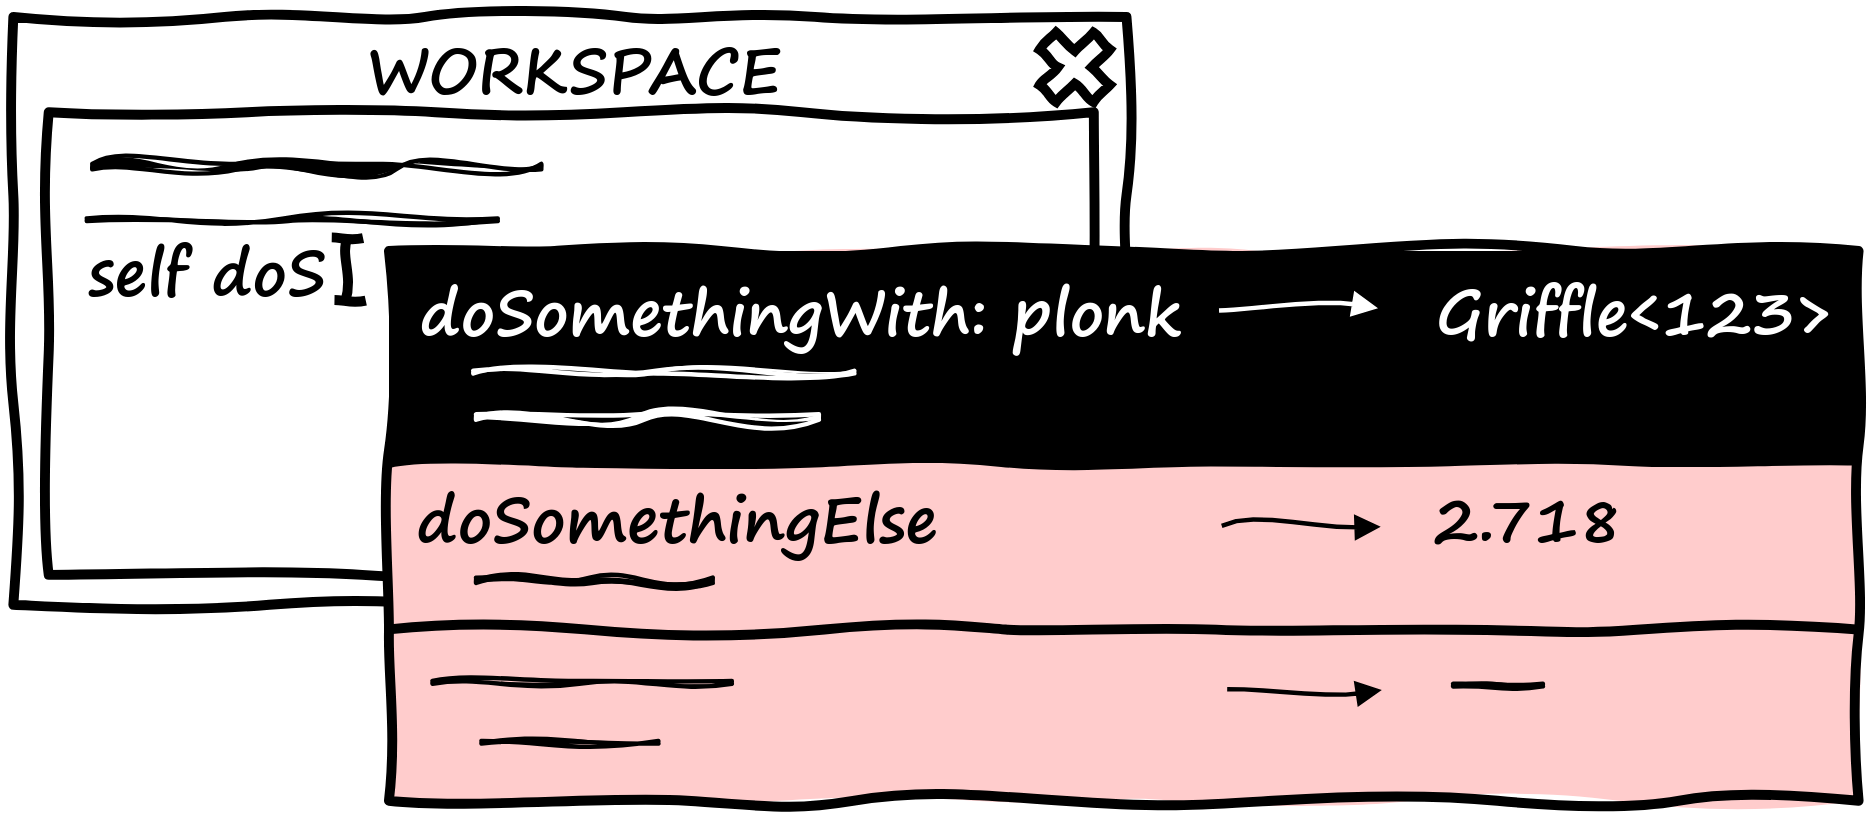
\includegraphics[width=\textwidth]{02_workspace/completions.png}
	\caption[TODO]{
		TODO
	}
	\label{fig:implementation/completions}
\end{figure}

For the user interface of completions, we use the \name{Autocompletion} package\footnote{\url{https://github.com/LeonMatthes/Autocompletion}} and employ its \code{ECEntryHook} interface~(\cref{fig:implementation/completions}).
We contribute two new types of completion entries: \emph{correlated identifiers} and \emph{generated expressions}.

First, we provide regular selectors and variable names based on correlated suggestion artifacts from the suggestion space and merge them with traditional \name{Autocompletion} entries.
This considers the original ranking of entries, which was only based on alphabetical order and most recently used date, and ehances it with their semantic relevance.
We hook into the presentation of entries to enrich suggested identifiers with usage information mined from their precending similar code artifacts as well as related documentation.

Second, we include contextualized generated expressions into the completion menu~(see \cref{sec:suggestions/generation}).
Analogously to the suggestion space, semantic completions are computed asynchronously in the background to avoid noticable delays in the user interface.

To generate a preview of the result of generated expressions, we run them in the editor context inside an isolated sandbox of \name{SimulationStudio} and include the results in the presentation of each entry.
